\subsection{Synthetic gates generation}

The process of generating a synthetic scene containing random meshes is done in
several steps.\\

In a first time, a virtual camera is initialized based on the real camera's intrinsic
parameters, from which a projection matrix can be derived.

In a second time, a random choice of available meshes is spawned in the virtual
scene, with random translations and rotations.

The final step is to compute the closest gate to the camera being in its field
of view, and project its center coordinates onto the image, so that a
ground truth label can be inferred.\\

\todo{Insert pseudo code of the algorithm}.

	\subsubsection{OpenGL scene}

The synthetic scene generation is implemented in OpenGL 3.3~\cite{OpenGL},
using the Python wrapper ModernGL~\cite{ModernGL}. \todo{Cite python?}
OpenGL is a cross-platform graphics library that is available in several
programming languages, and which allows rendering 2D and 3D vector graphics via
hardware acceleration. To be precise, OpenGL is merely a specification of how
every graphics card manufacturer should implement the API for the end users.

Using the OpenGL API removes the need to write the boilerplate necessary to
render polygons, and takes care of most low-level transformations that need to
happen before pixels are drawn on the screen.\\


OpenGL can basically be considered as a state machine handling objects, in the
form of C structures, and referred to as the context. It is important to know
that it is entirely independent of the operating system, and therefore does
not handle on-screen rendering. What needs to be understood is that OpenGL only
``renders'' things in a buffer, and it is the user's responsibility to
instantiate a window and draw that buffer's content inside it, so it can be
visible on a screen. That part is usually handled by other libraries to make
this task easier, however it is out of scope for this work, where the render
only needs to be saved to an image file.\\

The 3D to 2D transformation process is executed by OpenGL's graphics pipeline.
It mainly consists of two consecutive actions.

\begin{figure}[h]
	\center
	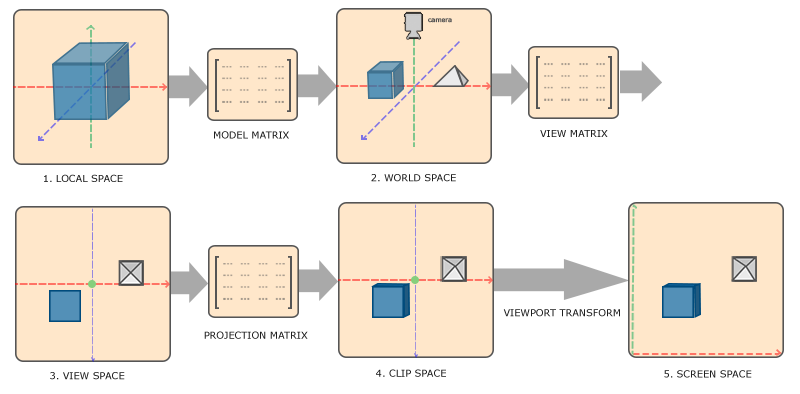
\includegraphics[width=0.99\textwidth]{figure/pipeline.png}
	\caption[OpenGL transformations pipeline]{The OpenGL transformations
	pipeline. Credits to learnopengl.com~\cite{LearnOpenGL} }
	\label{fig:openglpipeline}
\end{figure}

For the first step, 3D coordinates are transformed to be in the normalized
device coordinates space, which is in the [-1.0, 1.0] range and centered at the
origin. Coordinates that are outside this space will not be visible on screen.
The camera ``view'' matrix, derived from the extrinsic parameters is then used
to apply transformations to the world coordinates, so that objects appear to be
in front of the camera, from a relative point of view.

As for the second step, the projection matrix, derived from the view matrix and
the camera intrinsics, applies further transformations to give a sense of
perspective, by modeling a pin-hole camera model. Finally, the \emph{viewport
transform} (an OpenGL internal process) is in charge of transforming the 3D
coordinates from the range [-1.0, 1.0] to a range corresponding to the
specified viewport, which can be considered as the image resolution. The result
is sent to the rasterizer, the OpenGL process responsible for turning
coordinates into colored pixels.


	\subsubsection{Modeling the camera}

Having a base dataset of background images annotated with the drone translation
and rotation at every frame, it is trivial to model a camera in the exact same
configuration. The real camera mounted on the drone can be considered to have
the same pose as the drone, since it is only a few centimeters away from its
geometrical center. The motion capture system has been calibrated so that the
origin of the physical coordinates system is at that the center of the lab,
with a slight and negligible shift of a few centimeters.\\

\begin{figure}[h]
	\center
	\resizebox{280pt}{!}{
		
\pgfmathsetmacro{\viewtheta}{60}
\pgfmathsetmacro{\viewphi}{120}
\pgfmathsetmacro{\rvec}{5}
\pgfmathsetmacro{\thetavec}{60}
\pgfmathsetmacro{\phivec}{100}
\pgfmathsetmacro{\rvectarget}{5}
\pgfmathsetmacro{\thetavectarget}{90}
\pgfmathsetmacro{\phivectarget}{40}

\tdplotsetmaincoords{\viewtheta}{\viewphi}

\begin{tikzpicture}[scale=1,tdplot_main_coords]

% Base Coordinate System
\tdplotsetcoord{O}{0}{0}{0}
\tdplotsetthetaplanecoords{0}
\draw[thick,->] (0,0,0) -- (4,0,0) node[anchor=north east]{$x_{W}$};
\draw[thick,->] (0,0,0) -- (0,4,0) node[anchor=north west]{$y_{W}$};
\draw[thick,->] (0,0,0) -- (0,0,4) node[anchor=south]{$z_{W}$};


% First Coordinate System
\tdplotsetcoord{P}{\rvec}{\thetavec}{\phivec}
\draw[dashed,->,thick] (O) -- (P) node[near end,anchor=south]{$\mathbf{r}_{W}$};

\tdplotsetrotatedcoordsorigin{(P)}
%\tdplotsetthetaplanecoords{40}
\tdplotsetrotatedcoords{20}{10}{20}
\draw[thick,tdplot_rotated_coords,->] (0,0,0) -- (1.5,0,0) node[anchor=north
  west]{$x_{B}$};
\draw[thick,tdplot_rotated_coords,->] (0,0,0) -- (0,1.5,0) node[anchor=west]{$y_{B}$};
\draw[thick,tdplot_rotated_coords,->] (0,0,0) -- (0,0,1.5) node[anchor=west]{$z_{B}$};
%% Draw Up Vector
\draw[blue,-stealth,dashed,tdplot_rotated_coords] (0,0,0) -- (0,0,3)
  node[anchor=south]{$\mathbf{u}_{B}$};


\tdplotsetcoord{B}{11}{80}{59.5}
\tdplotsetrotatedcoordsorigin{(B)}
\shade[ball color=red,tdplot_rotated_coords] (0,0,0) circle (0.1cm);

% Draw Target Vector
\draw[red,-stealth,dashed,->,thick] (P) -- (B)
  node[anchor=north west,midway]{$\mathbf{t}_{B}$};

\draw[red,-stealth,dashed,->,thick] (O) -- (B) node[anchor=north,midway]{$\mathbf{t}_{W}$};


\end{tikzpicture}

	}
	\caption{World frame and body frame camera coordinates.}
	\label{fig:coordinatesystem}
\end{figure}

As shown on figure~\ref{fig:openglpipeline}, several transformations happen
before objects are rendered with perspective on the image frame. In OpenGL, it
is important to know that the camera is considered to be the center of the
world, in a fixed position and looking at the $-Z$-axis, while every object in
the world moves around it. The complete transformation which moves the objects
around, and virtually moves the camera around, is expressed as follows:

\begin{equation} \label{equ:opengltransform}
	M_{ModelViewProjection} = M_{projection} M_{view} M_{model}
\end{equation}

~\\In this section, the $M_{view}$ and $M_{projection}$ matrix are defined.

First of all, the way the $M_{view}$ matrix is usually created is by using a
function commonly available in OpenGL wrappers and other computer graphics math
libraries, such as \pyth{look_at(eye, target, up)} from the Python library
\emph{Pyrr}~\cite{Pyrr}.

\begin{figure}[h]
	\center
	\begin{python}
		# Camera view matrix
		view = Matrix44.look_at(
			# eye: position of the camera in world coordinates
			self.drone_pose.translation,
			# target: position in world coordinates where the camera is looking at
			self.drone_pose.translation + (self.drone_pose.orientation *
										   Vector3([1.0, 0.0, 0.0])),
			# up: up vector of the camera.
			self.drone_pose.orientation * Vector3([0.0, 0.0, 1.0])
		)
	\end{python}
	\caption[The \pyth{look_at()} function]{Creating the view matrix via the
	convenience \pyth{look_at()} function.}
\end{figure}

What the \pyth{look_at()} function does, is combining two transformations
inversely: first the camera is translated from the eye position to the origin,
then it is rotated from its orientation inferred from the target and up vectors
towards the $-Z$-axis at the origin.\\

It takes three arguments: the eye, the target, and the up vector. The eye is
basically the position of the camera in the world frame, which corresponds to
the drone position in the physical space. The target is a point in space where
the camera is looking at; it is represented by the $\mathbf{t}_W$ and
$\mathbf{t}_B$ vectors in figure~\ref{fig:coordinatesystem}, and calculated by the
Hamilton product of the drone orientation quaternion with a unit vector on the
$X$-axis (as to be in front of the field of view) in the body frame, added to
the drone translation in the world frame.

\begin{equation} \label{equ:targetvector}
	\mathbf{t}_W = \mathbf{r}_W + \mathbf{q}_B^W\:\mathbf{\hat{x}}_B\:
	(\mathbf{q}_{B}^{W})^{-1}
\end{equation}

Finally, the up vector is a simple unit vector orthogonal to the camera's
target vector, and calculated by the Hamilton product of the drone orientation
quaternion and an unit vector on the $Z$-axis. It is used to compute the
rotation matrix composing the final view matrix, $M_{view}$.

\begin{equation} \label{equ:upvector}
	\mathbf{u}_W = \mathbf{r}_W + \mathbf{q}_B^W \:\mathbf{\hat{z}}_B\:
	(\mathbf{q}_B^W)^{-1}
\end{equation}

~\\Under the hood, the \pyth{look_at()} function constructs the view matrix
as a composition of a translation and a rotation matrix, expressed as such:

\begin{equation} \label{equ:viewmatrix}
	M_{view} = M_R M_T = \begin{bmatrix}
							r_0 & r_4 & r_8 & 0\\
							r_1 & r_5 & r_9 & 0\\
							r_2 & r_6 & r_10 & 0\\
							0 & 0 & 0 & 1
						\end{bmatrix}
						\begin{bmatrix}
							1 & 0 & 0 & t_x\\
							0 & 1 & 0 & t_y\\
							0 & 0 & 1 & t_z\\
							0 & 0 & 0 & 1
						\end{bmatrix}
					=
						\begin{bmatrix}
							r_0 & r_4 & r_8 & r_0 t_x + r_4 t_y + r_8 t_z\\
							r_1 & r_5 & r_9 & r_1 t_x + r_5 t_y + r_9 t_z\\
							r_2 & r_6 & r_10 & r_2 t_x + r_6 t_y + r_10 t_z\\
							0 & 0 & 0 & 1
						\end{bmatrix}
\end{equation}

where $M_T$ is
\begin{equation}
	M_T = \begin{bmatrix}
			1 & 0 & 0 & -t_W_x\\
			0 & 1 & 0 & -t_W_y\\
			0 & 0 & 1 & -t_W_z\\
			0 & 0 & 0 & 1
		\end{bmatrix}
\end{equation}

and $M_R$ is
\begin{equation}
	M_R = \begin{bmatrix}
			l_x & u_x & f_x & 0\\
			l_y & u_y & f_y & 0\\
			l_z & u_z & f_z & 0\\
			0 & 0 & 0 & 1
		\end{bmatrix}^{-1}
		= \begin{bmatrix}
			l_x & u_x & f_x & 0\\
			l_y & u_y & f_y & 0\\
			l_z & u_z & f_z & 0\\
			0 & 0 & 0 & 1
		\end{bmatrix}^{T}
		= \begin{bmatrix}
			l_x & l_y & l_z & 0\\
			u_x & u_y & u_z & 0\\
			f_x & f_y & f_z & 0\\
			0 & 0 & 0 & 1
		\end{bmatrix}
\end{equation}

\todo{Add derivation in appendix?}
~\\Note the inverse of $M_R$ in the first step: as state above, the world is
rotated and translated \emph{around the camera}, while the latter faces the
$-Z$-axis.\\

The only thing left to do is to transform the normalized device coordinates
into the eye coordinates, also called \emph{frustum}, in order to apply a
perspective projection.

The projection matrix, $M_{projection}$, is responsible for the pin-hole
modeling of the camera (described on figure~\ref{fig:pinholemodel}), and
creating this perspective illusion rendered on a 2D surface. It is defined as

\begin{equation} \label{equ:projection}
	P = \begin{bmatrix}
			\cfrac{f_x}{c_x} & 0 & 0 & 0 \\
			0 & \cfrac{f_y}{c_y} & 0 & 0 \\
			0 & 0 & \cfrac{-z_{far} -z_{near}}{z_{far} - z_{near}} & -1\\
			0 & 0 & \cfrac{-2 \, z_{far} z_{near}}{z_{far}-z_{near}} & 0
		\end{bmatrix}
\end{equation}

~\\with $f_x$ and $f_y$ being the focal lengths in pixels, $c_x$ and $c_y$ the
principal point coordinates in pixels (usually at the image center), and
$z_{far}$ and $z_{near}$ being the clip space distances. Those values are
obtained by calibrating the drone's camera~\cite{OpenCVCalibration}, which
means they can only reflect a specific pin-hole model of a unique camera. Refer
to figure~\ref{fig:pinholemodel} for a more visual representation of the
projection.

\begin{figure}[h]
	\center
	\resizebox{350pt}{!}{
		\usetikzlibrary{calc,arrows.meta,positioning,backgrounds}
\tdplotsetmaincoords{-60}{-35}
\begin{tikzpicture}
  [
    tdplot_main_coords,
    >=Stealth,
    my dashed/.style={dashed, thick, ->, shorten >=-15pt, shorten <=-15pt, every node/.append style={font=\footnotesize}},
    my box/.style={thin, gray!70},
    my blue/.style={blue, line cap=round, -{Triangle[width=3*#1]}, line width=#1, shorten >=#1*1.75pt, every node/.append style={fill, circle, inner sep=0pt, minimum size=#1*3.5pt, anchor=center, outer sep=0pt}},
    my label/.append style={midway, font=\scriptsize},
    my vectors/.style={green!50!black, {Stealth[scale=.75]}-{Stealth[scale=.75]}},
    my red/.style={thick, red, line cap=round},
    my grey/.style={gray!70},
    description/.style={draw=gray!70, thick, line cap=round, every node/.style={align=center, font=\scriptsize\sffamily, anchor=north}},
  ]
%   \draw [help lines] (-2,0,0) -- (2,0,0) node[anchor=north west]{$x$} (0,0,0) -- (0,7,0) node[anchor=north east]{$y$} (0,0,0) -- (0,0,2) node[anchor=north]{$z$} (-2,7,0) -- (2,7,0);
  \draw [my grey] (0,4,0) -- (0,7,0) (-2,7,0) -- (2,7,0);
  \coordinate (o) at (0,0,0);
  \path [draw=gray!70, text=gray, fill=gray!20, opacity=0.8, text opacity=1] (-1.5,4,1.75) coordinate (a) -- ++(0,0,-3.5) coordinate (b) -- ++(3,0,0) coordinate (c) -- ++(0,0,3.5) coordinate (d) -- cycle node [pos=.95, above, sloped, anchor=south west] {$z=f$} ;
%   \foreach \i in {a,b,c,d} \node [red, font=\scriptsize] at (\i) {\i};
  \draw [my grey] (-2,0,0) -- (2,0,0) (0,0,0) -- (0,4,0) (0,0,0) -- (0,0,2);
  \draw [thick, ->, every node/.style={font=\footnotesize, inner sep=0pt}] (o) node [anchor=north west] {$F_c$} (o) edge node [pos=1, anchor=north east] {$z_c$} ++(0,1,0) edge node [pos=1, anchor=north] {$y_c$} ++(0,0,1) -- ++(1,0,0) node [anchor=north west] {$x_c$};
  \draw [my box] (o) ++(0,4,-.5) coordinate (p1) -- ++(1,0,0) coordinate (p2) -- ++(0,0,-1.25) coordinate (p3);
  \foreach \i in {0,1,...,4} \draw [my box] (p1) ++(\i*.25,0,0) -- ++(0,0,-.25);
  \foreach \i in {0,1,...,5} \draw [my box] (p2) ++(0,0,-\i*.25) -- ++(-.25,0,0);
  \draw [my box] (p1) ++(0,0,-.25) -- ++(.75,0,0) -- ++(0,0,-1);
  \draw [my dashed, cyan] ($(b)!1/2!(c)$) -- ($(d)!1/2!(a)$) node [below=15pt, anchor=north] {$y$};
  \draw [my dashed, cyan] ($(b)!1/2!(a)$) -- ($(d)!1/2!(c)$) node [above right=17pt, anchor=north west] {$x$};
  \draw [my dashed, green!50!black, <->] (a) node [below=15pt, anchor=north] {$v$} -- (b) -- (c) node [above right=17pt, anchor=north west] {$u$};
  \path [green!50!black, every node/.style={font=\scriptsize, inner sep=0pt}] (p2) node [above right, anchor=south west] {$(u,v)$};
  \path (p2) ++(-.125,0,0) coordinate (q2) ++(0,0,-.125) coordinate (r2);
  \draw [my blue=1] ($(0,4,0)+($(q2)-(p1)$)$) coordinate (s2) -- (r2) node (d1) {};
  \scoped[on background layer]{\draw [my blue=1.75] ($($1.75*($(s2)-(0,4,0)$)$)+(0,7,0)$) -- ++($1.75*($(r2)-(s2)$)$) node (d2) [label={[label distance=-20pt]above:{$P=(X,Y,Z)$}}] {};}
  \draw [my vectors] (0,4,.1) -- ($(s2)+(0,0,.1)$) node [below, my label, sloped] {$\vec{u}$};
  \draw [my vectors] (-.1,4,0) -- ($(q2)-(s2)+(-.1,4,0)$) node [left, my label] {$\vec{v}$};
  \draw [my red] (o) -- (d1.center);
  \scoped[on background layer]{\draw [my red] (d1.center) -- (d2.center);}
  \path [description] (0,4,0) [out=-95, in=95] to (-.75,4,.25) node
  {principal\\point} (0,6.5,0) [out=-95, in=95] to (-.75,6.5,.25) node
  {vanishing\\point};
\end{tikzpicture}

	}
	\caption[Pin-hole camera model]{The pin-hole camera model. Credits to
	\cite{cfr}.}
	\label{fig:pinholemodel}
\end{figure}


	\subsubsection{Mapping a virtual space}

Once the camera is modeled and is positioned in the virtual scene so
that it matches the real world conditions, each randomly picked 3D mesh is
translated and rotated in the scene. By applying random transformations, the
algorithm aims to recreate unique combinations of drone racing circuits for
each frame. As a result, it is possible, and often the case, that only a small
subset of the originally selected meshes are visible on the image frame
(depending on the camera pose), or even none at all. For instance, if an
extracted frame from the base dataset indicates that the drone is facing a wall
up close, it would make sense not to render any gates at all, to preserve
coherence.\\

In order to achieve this, the virtual scene is constrained within boundaries
that match the physical environment in which the background images were
recorded. The origin of the motion capture system being roughly at the center
of the premise, it is trivial to set boundaries around the origin of the
virtual world, that match the ones of the physical environment.\\

The model transformation matrix of equation~\refer{equ:opengltransform} is a
combination of a translation and a rotation (note the importance of the order
of the transformations), defined by the Hamilton product between $M_T$ and $q$
as

\begin{equation} \label{equ:modelmatrix}
	M_{model} = M_T q 
\end{equation}

where $M_T$ is a $4 \times 4$ matrix inferred from a 3D vector where the $X$
and $Y$ components are randomly chosen within the world boundaries, and $Z$ is
set to 0 as to keep the gate on the ground level. As for $q$, it is quaternion
calculated by a rotation around the $Z$-axis, as a random factor of Pi, so that
it stays vertically placed on the ground.

In addition, a constraint is added to the translation vector of each gate, in
order to ensure that a minimum distance is kept between all of them. This is
done by re-computing the randomized vector until the Euclidean distance between
every gate is above a certain threshold.\\

On a last note, it must be acknowledged that there is no unit of measurement in
OpenGL. Indeed, it is the programmer's responsibility to define such unit, and
design a world according to that choice.

To reproduce the same scale as the real gates and arena, it is necessary to
model the meshes with a unit that is relative to the one used to position the
camera in 3D space.

	\subsubsection{Annotating}

The annotations for each image consist mainly of the \textbf{nearest}
gate's center coordinates in pixels, as well as a boolean for the
visibility of a gate \textbf{center} in the image frame.

First of all, the closest gate to the camera, that is in the clip space, has to
be selected. To do so, the Euclidean norm between the camera and the gate
center is used as a first metric. The gate center coordinates are inferred by
adding the base mesh translation vector $[x, y, 0]$ to another 3D vector
representing the center of the gate, and given in a configuration file after
modeling the mesh.

In addition, the gate center's world coordinates are projected onto the image
plane (in the clip space) to determine whether the gate is visible or not. This
is done by applying the $M_{ModelViewProjection}$ transformations matrix to the
world coordinates, and manually clipping the resulting coordinates if needed.

\todo{Add homogeneous vs orthogonal coordinates in clip space?}

To do so, the resulting 4D vector of homogeneous coordinates is simply divided,
element-wise, by its last component (usually called $w$) if that one is not
equal to zero: that operation is called \emph{projection divide}. This results
in a 3D vector of Cartesian coordinates in the normalized device space (within
the range $[1.0, 1.0]$).

Finally, a last transformation is needed to obtain image frame coordinates (in
pixel units), the \emph{viewport transform}:

\begin{equation}
	\begin{bmatrix}
		x_w\\y_w
	\end{bmatrix}
	=
	\begin{bmatrix}
		\cfrac{w}{2} x_{ndc} + (x + \cfrac{w}{2})\\
		\cfrac{h}{2} y_{ndc} + (y + \cfrac{h}{2})\\
	\end{bmatrix}
\end{equation}

where $x_w$ and $y_w$ are the gate center coordinates in the window
frame (or image) and $x_{ndc}$ and $y_{ndc}$ in the normalized device
coordinate system, $w$ and $h$ are the width and height of the view port -- or
the output image frame -- and $x$ and $y$ correspond to the viewport offset in
pixels, which are initially set to 0.\\

Furthermore, to improve the correctness of the annotations and follow a human
logic, an out-of-screen tolerance percentage is added to select a target gate
even if its center is slightly outside of the viewport. In that way, the
intuition of targetting a gate which is clearly visible, but whose center does
not seem to be in the field of view , can be applied to the network.\\

For future improvements, the gate rotation is also computed, with respect to
the camera. This is done by rotating the mesh by a factor of Pi when it is
spawned in the scene, if the cross product between the camera's vector and the
line crossing the gate in the $X$-axis results in a vector whose $Z$ axis is
negative.
